\documentclass{ctexart}  
\usepackage[left=2cm,right=1.97cm,top=2cm,bottom=2cm]{geometry}	
\usepackage{ctex}
\usepackage{palatino}
\usepackage{lipsum}
\usepackage{graphicx}
\usepackage{hyperref}
\usepackage{tabularray}
\usepackage{color}
\usepackage{listings}
\usepackage{float}
\usepackage{xcolor}
\usepackage[longtable]{multirow}
\usepackage{longtable}
\title{\heiti \zihao{2}实验三:调试及性能分析、元编程演示实验、PyTorch编程学习实验报告}
\author{\kaishu \zihao{-4} 邓林\qquad 23020007014\\
\songti \zihao{-5}中国海洋大学 \qquad 23软件工程 }
\date{}
\ctexset{section={format={\heiti \zihao{4}}},
subsection={format={ \songti \zihao{4}},beforeskip=0pt,afterskip=0pt},
subsubsection={format={\kaishu \zihao{4}},beforeskip=0pt ,afterskip=0pt}}
%%%%%%%%%%%%%%%%%%%%%%%%%

\begin{document}
    \maketitle
\vspace{-20pt}\begin{abstract}				
    本实验报告主要记录了作者通过课程网站及B站学习调试及性能分析、
    元编程演示实验、
    PyTorch编程的学习过程以及心得。
\end{abstract}

\section{实验内容}
\begin{longtable}{cl} 
    \hline
    \multicolumn{2}{c}{pdb指令}                              \endfirsthead 
    \hline
    python -m pdb filename & 进入pdb                         \\
    list/l                 & 显示当前行附近的 11 行或继续执行之前的显示       \\
    list ./l .             & 列出当前函数的代码                     \\
    long list/ll           & 显示所有代码                        \\
    next/n                 & 继续执行直到当前函数的下一条语句或者 return 语句  \\
    step/s                 & 执行当前行,并在第一个可能的地方停止            \\
    continue/c             & 执行代码到下一个断点                    \\
    break 文件行数             & 设置断点(基于传入的参数)                 \\
    break                  & 显示所有断点                        \\
    cl 序号                  & 清除指定断点                        \\
    cl                     & 清除所有断点                        \\
    disable                & 暂停使用指定断点                      \\
    enable~                & 恢复使用指定断点                      \\
    until 行号               & 执行代码到指定行号                     \\
    p                      & 在当前上下文对表达式求值并打印结果             \\
    r                      & 继续执行直到当前函数返回                  \\
    q                      & 退出调试器                         \\
    \hline
    \end{longtable}

\subsection{调试及性能分析}
\begin{enumerate}
    \item 使用日志
\begin{figure}[H]
    \centering
    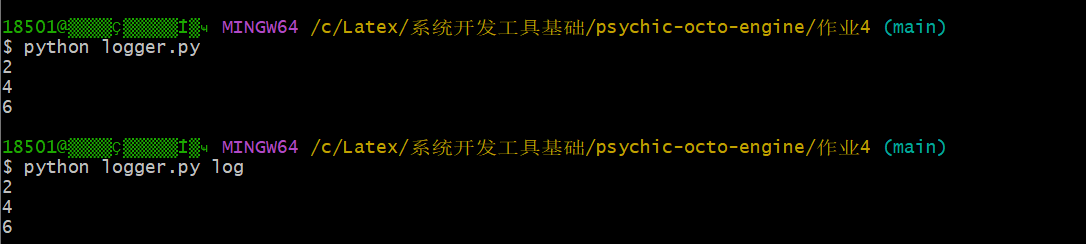
\includegraphics[width=14cm]{f0c8daaa91bc8a6d4159431336a4f244.png}
    \caption{空 和 log}
    \label{fig:1}
\end{figure}

\begin{figure}[H]
    \centering
    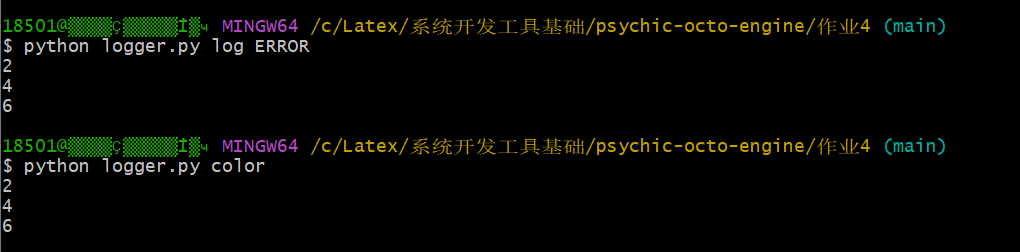
\includegraphics[width=14cm]{9571e16dc29fad803d55cc2b24eee718.png}
    \caption{log ERROR 和 color}
    \label{fig:2}
\end{figure}

\item 改变输出结果的颜色
\begin{figure}[H]
    \centering
    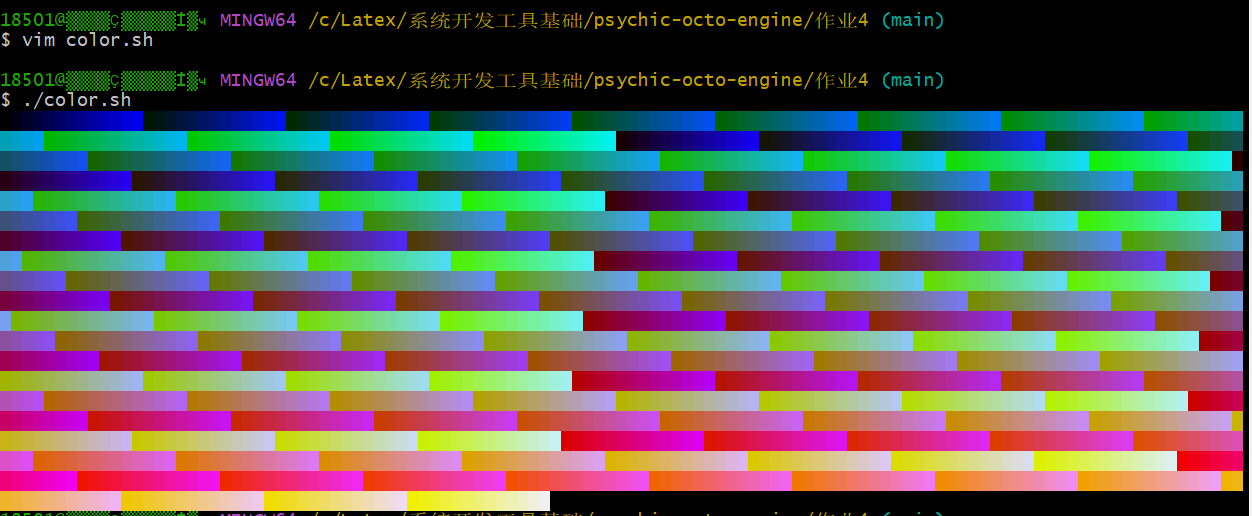
\includegraphics[width=14cm]{9cc3029c117e11aaf23ab16a4da10899.png}
    \caption{在终端中打印多种颜色}
    \label{fig:3}
    \end{figure}
\end{enumerate}




\subsection{PyTorch编程}
\begin{enumerate}
\item 下载PyTorch并配置环境,调试
\begin{figure}[H]
    \centering
    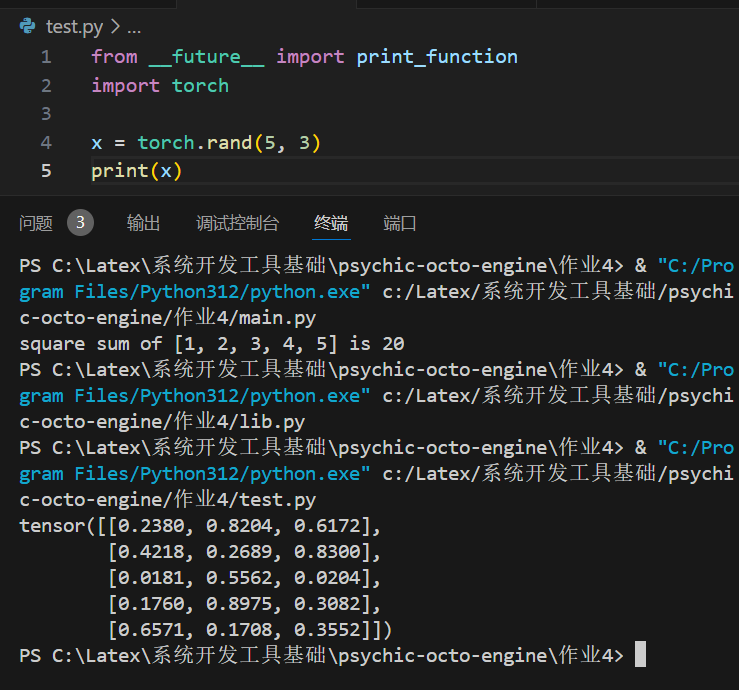
\includegraphics[width=14cm]{04b85f81e2ad45d4282cce5fbfb0b2cf.png}
    \caption{安装PyTorch}
    \label{fig:20}
    \end{figure}
    \item 张量(Tensors)
    \begin{figure}[H]
    \centering
    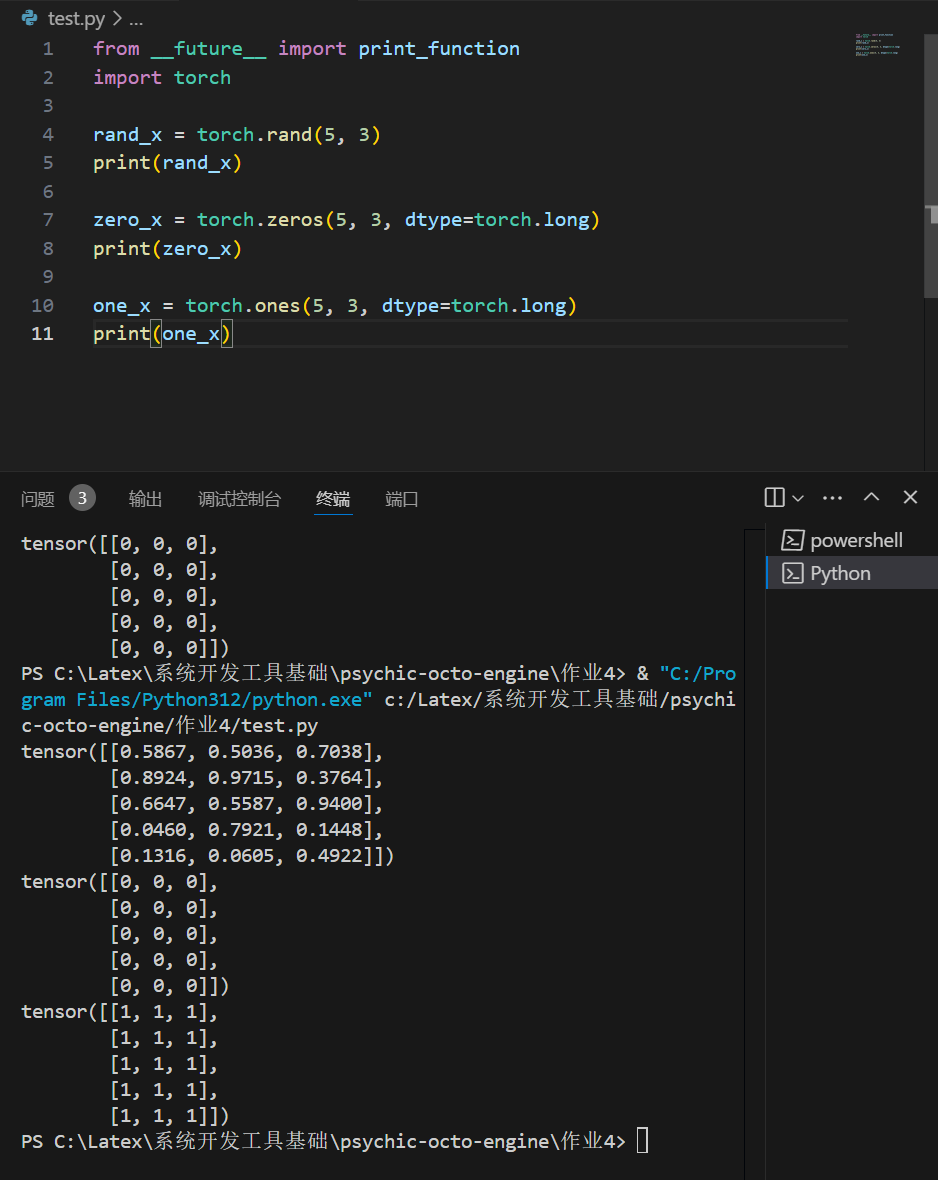
\includegraphics[width=14cm]{814323ed910b56b4a117fd3af5aa29e2.png}
    \caption{torch.zeros():创建数值皆为 0 的矩阵}
    \label{fig:21}
    \end{figure}
    \item 操作(Operations)
    \begin{figure}[H]
    \centering
    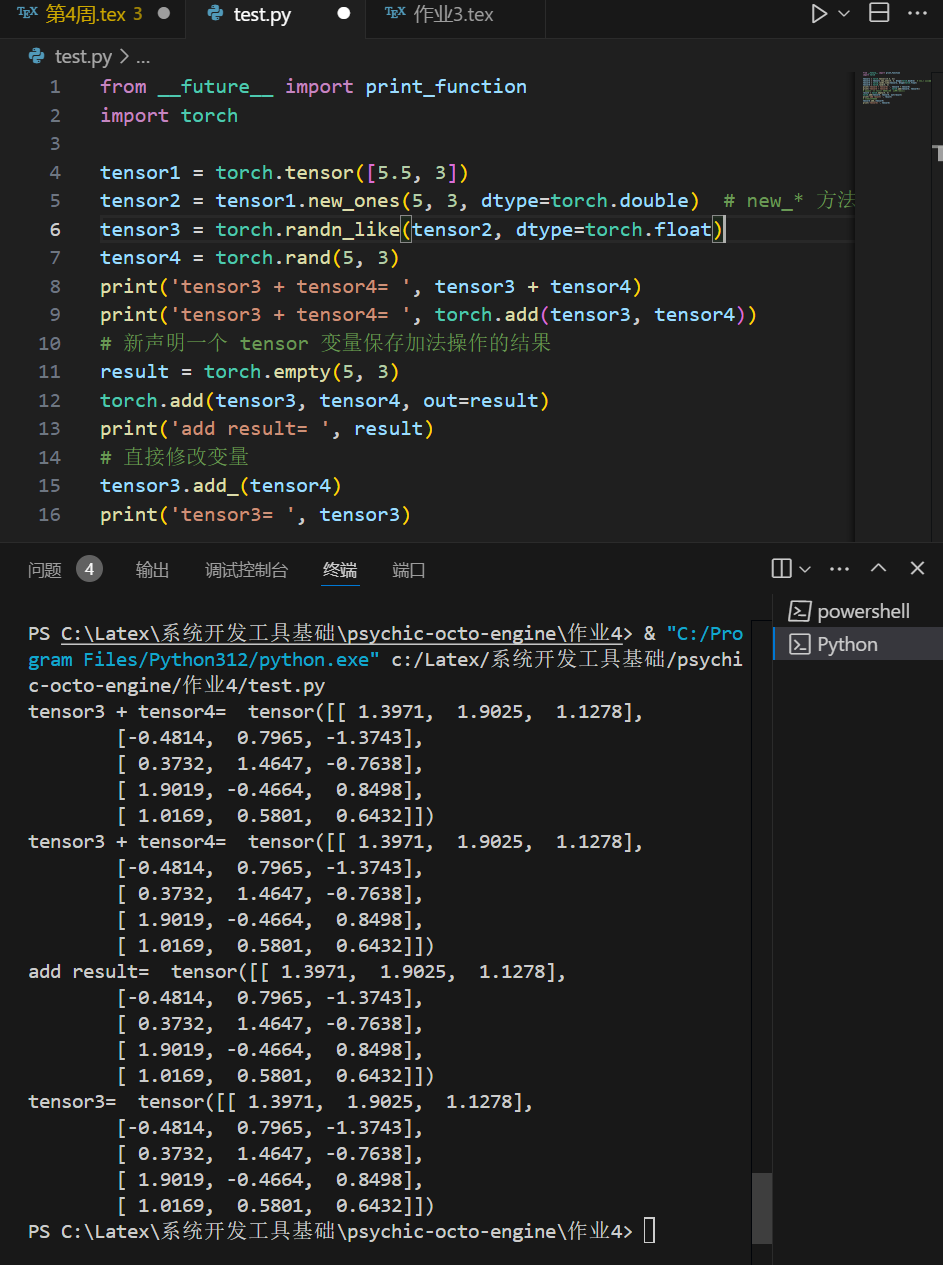
\includegraphics[width=14cm]{e93972feeca18128e84d6c23e700a704.png}
    \caption{效果如图}
    \label{fig:22}
    \end{figure}
    \item 和 Numpy 数组的转换
    \begin{figure}[H]
    \centering
    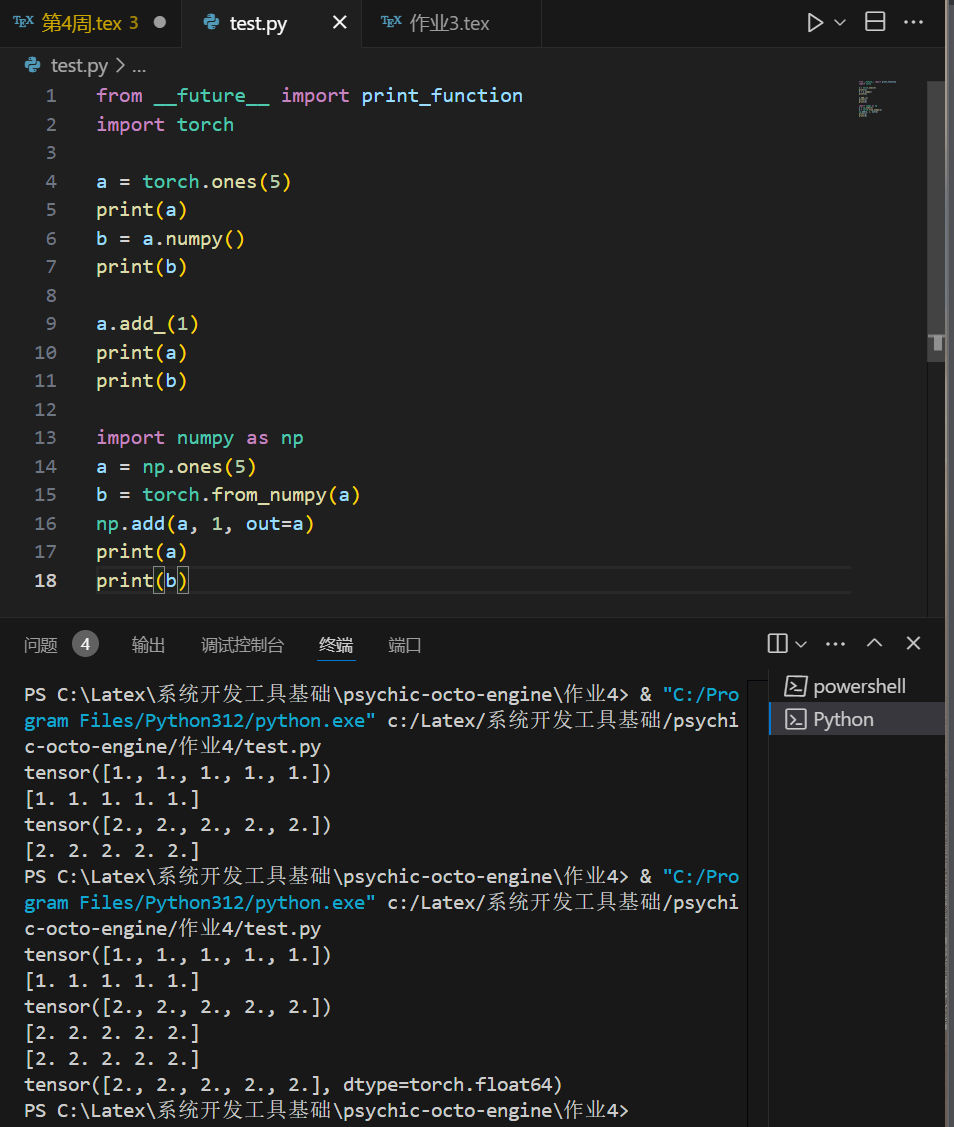
\includegraphics[width=14cm]{8273c8f228e59438002d136c2c3a9186.png}
    \caption{效果如图}
    \label{fig:23}
    \end{figure}
    \item CUDA 张量
    \begin{figure}[H]
    \centering
    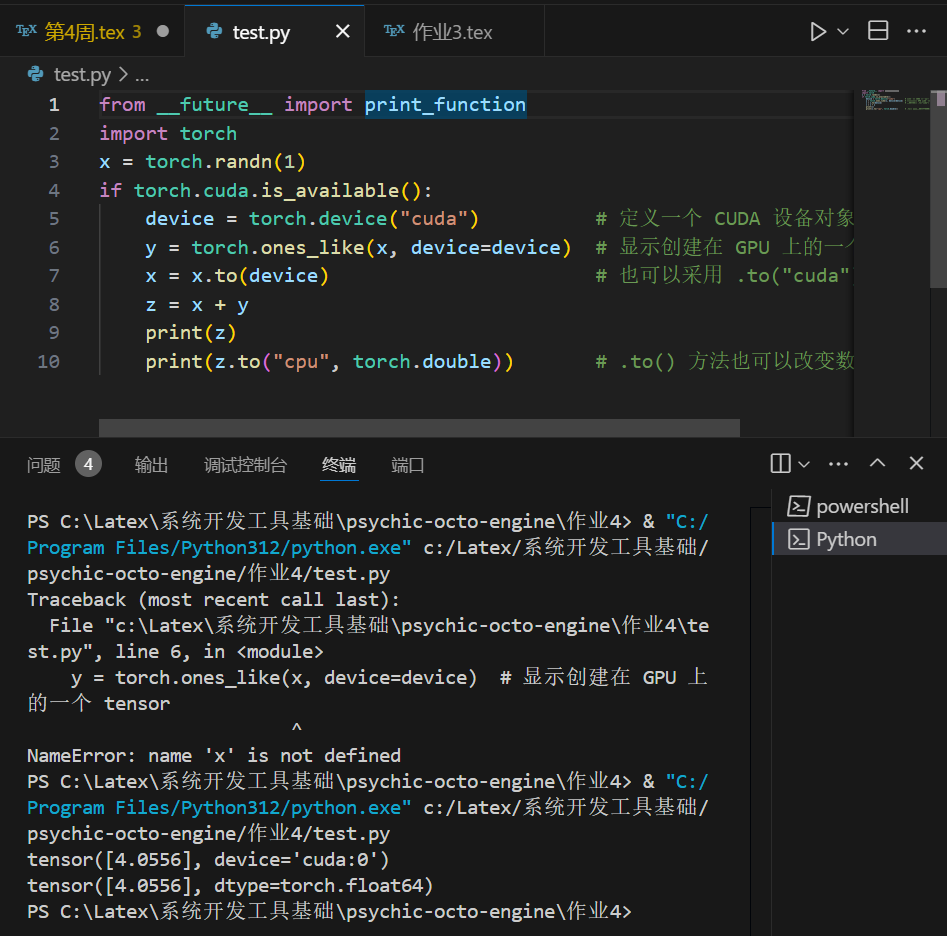
\includegraphics[width=14cm]{7a55f75441832367e6e3ff0ee92cff49.png}
    \caption{效果如图}
    \label{fig:23}
    \end{figure}
    \item autograd 张量
    \begin{figure}[H]
    \centering
    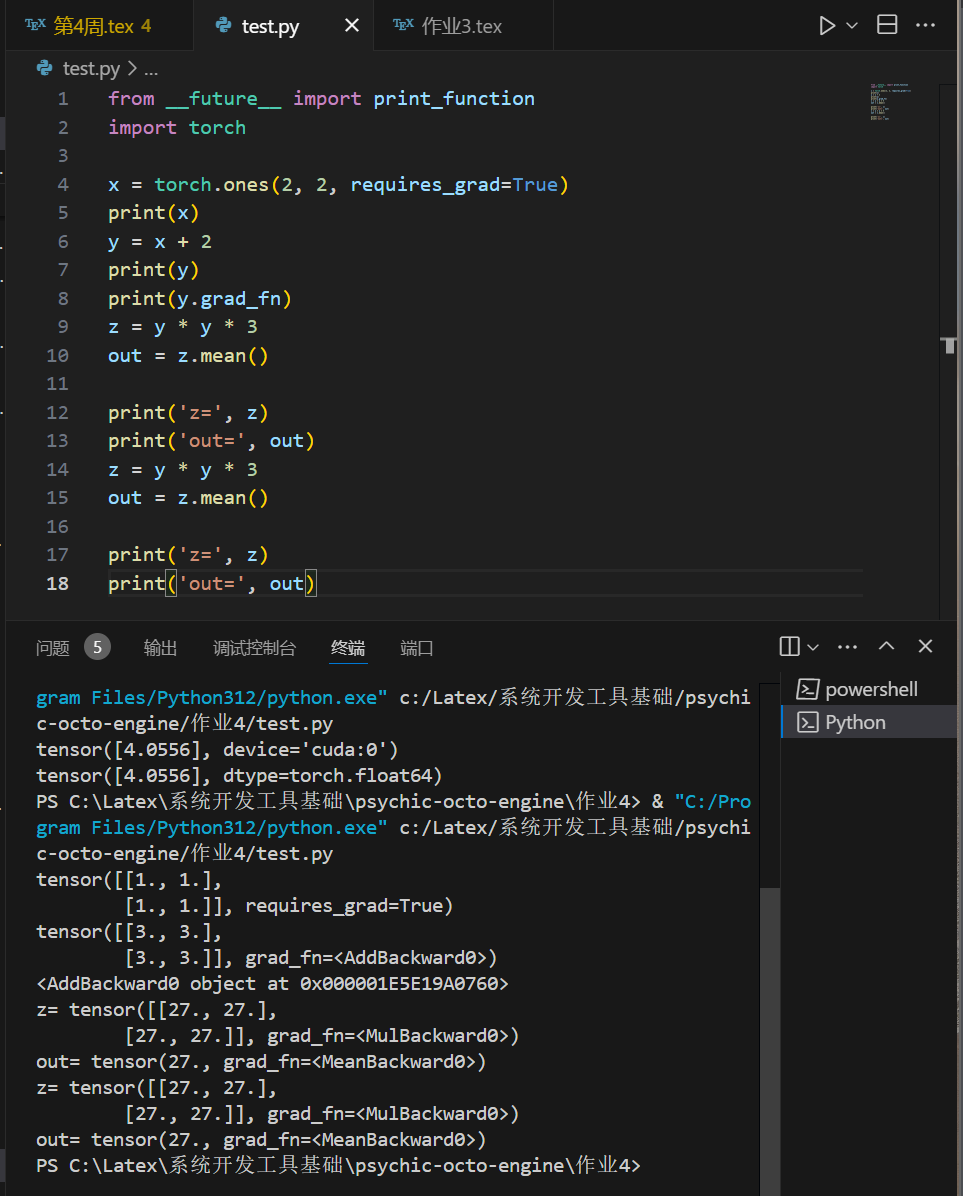
\includegraphics[width=14cm]{a97225869c464ad9325103a09b31a3f8.png}
    \caption{效果如图}
    \label{fig:23}
    \end{figure}
    \item 梯度
    \begin{figure}[H]
    \centering
    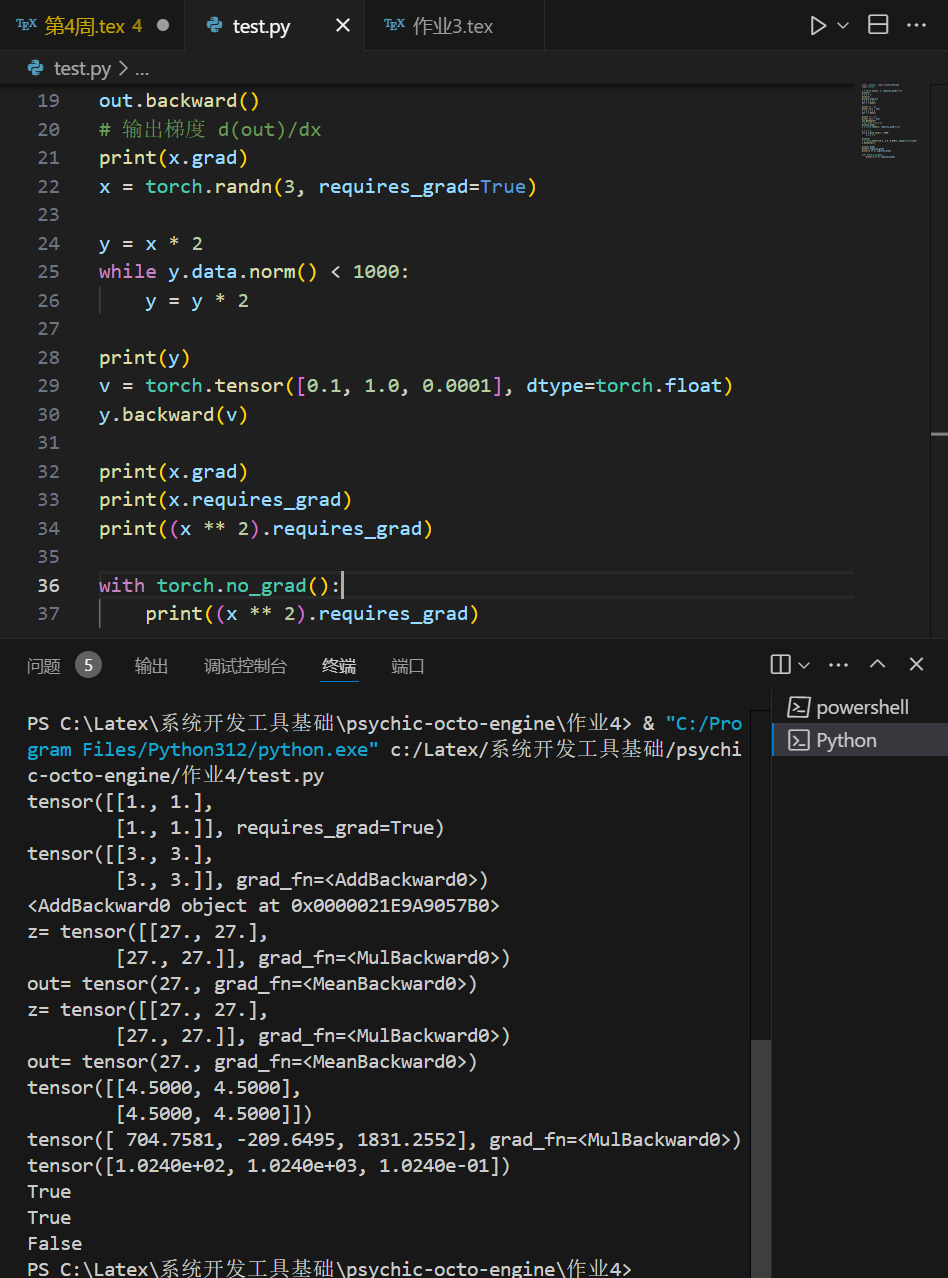
\includegraphics[width=14cm]{6ce332ebb8898a533effba33b7979268.png}
    \caption{效果如图}
    \label{fig:23}
    \end{figure}
\end{enumerate}


\section{课后习题}
\subsection{调试及性能分析}
\begin{enumerate}
    \item 使用 Linux 上的 journalctl 或 macOS 上的 log show 命令来获取最近一天中超级用户的登录信息及其所执行的指令。
    \begin{figure}[H]
        \centering
        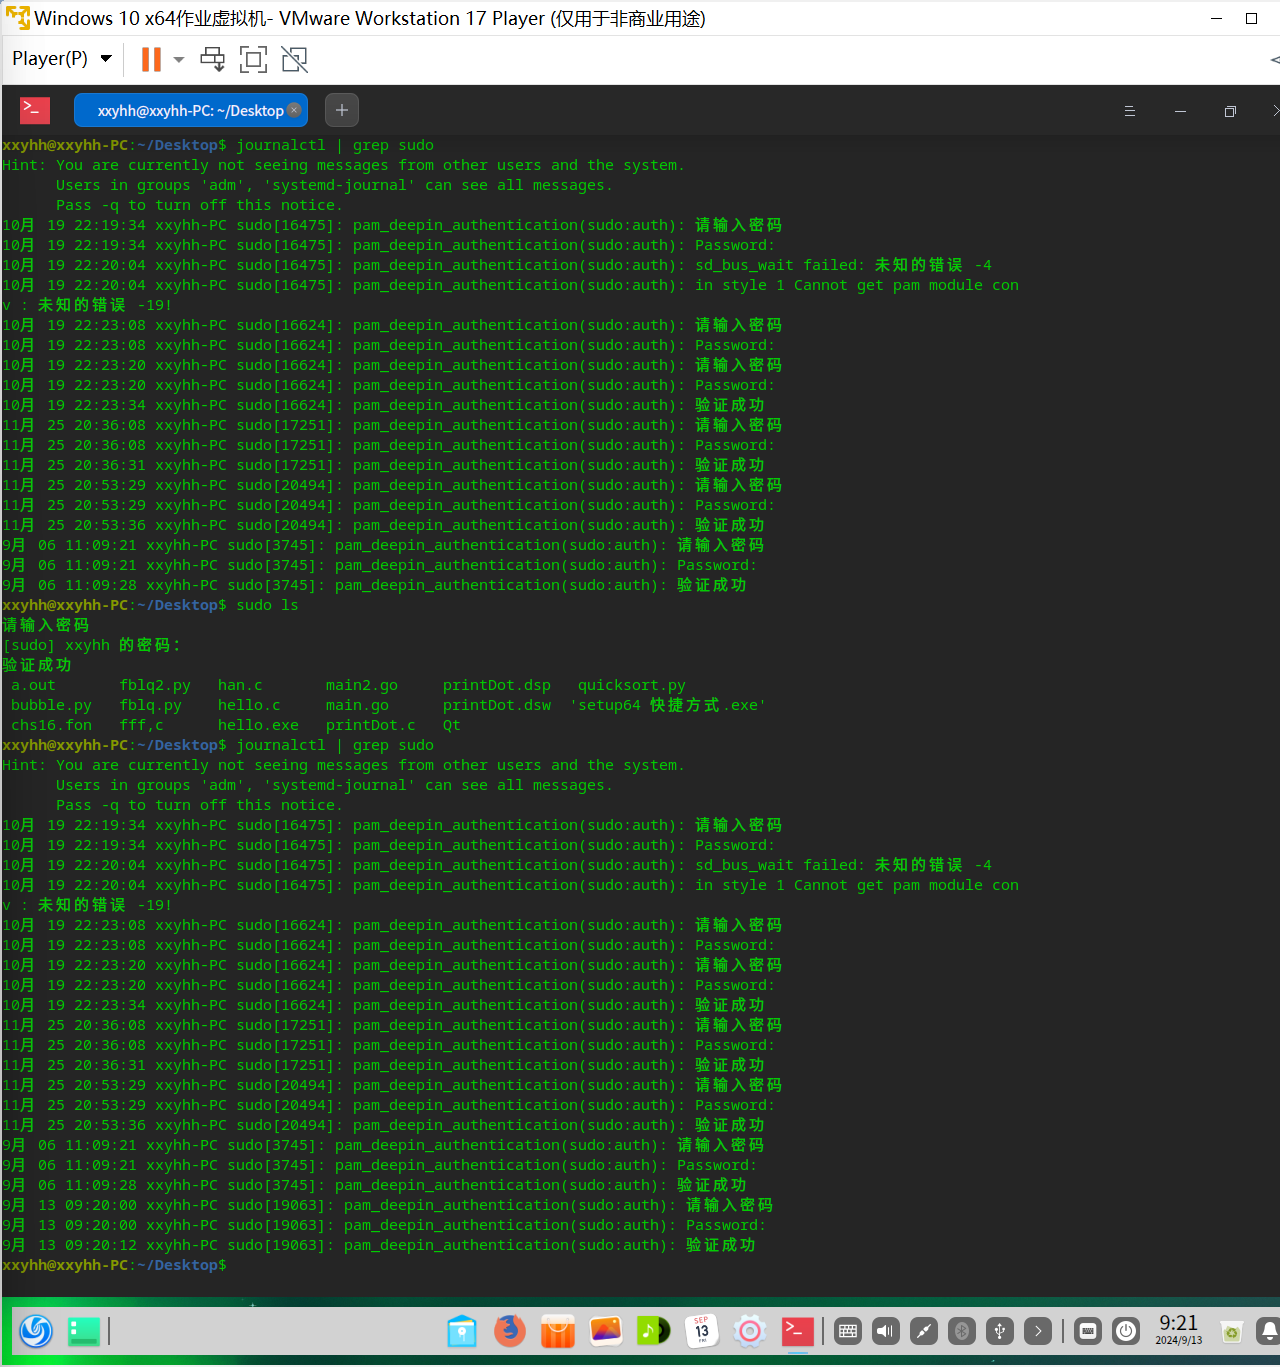
\includegraphics[width=12cm]{8bb31c175076ac6358f1ea10075020ac.png}
        \caption{在终端中打印多种颜色}
        \label{fig:4}
        \end{figure}

    \item pdb学习
    1.首先我们编写了一个函数,用于计算算术平方和,在main函数中调用函数计算1-5的平方和:
    \begin{figure}[H]
        \centering
        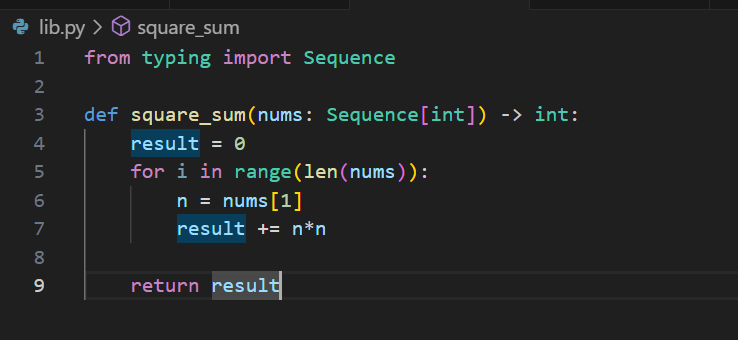
\includegraphics[width=12cm]{f4af56aefc982f41246adb38af28c064.png}
        \caption{lib.py}
        \label{fig:5}
        \end{figure}
     \begin{figure}[H]
        \centering
        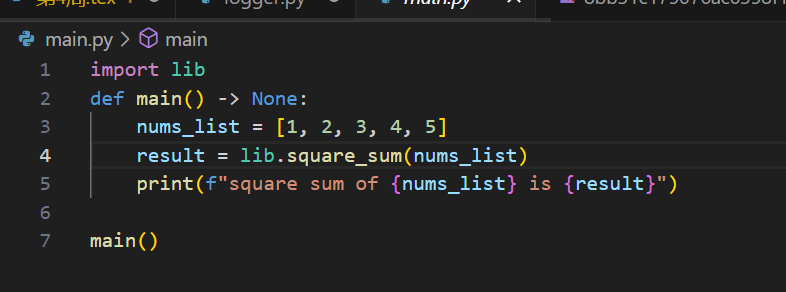
\includegraphics[width=14cm]{14f60fcd64dc0bf5d36fb2a7a9dc5adb.png}
        \caption{main.py}
        \label{fig:6}
        \end{figure}   
    2.运行发现答案不符合预期
    \begin{figure}[H]
        \centering
        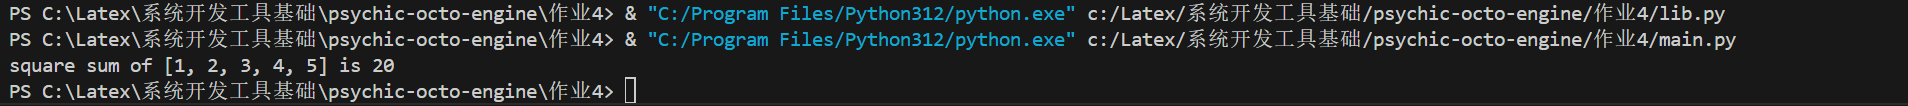
\includegraphics[width=14cm]{5fd6b435237099e54b69e634f0264935.png}
        \caption{运行结果}
        \label{fig:7}
        \end{figure}   

    3.这时我们打开终端利用pdb调试代码
    \begin{figure}[H]
        \centering
        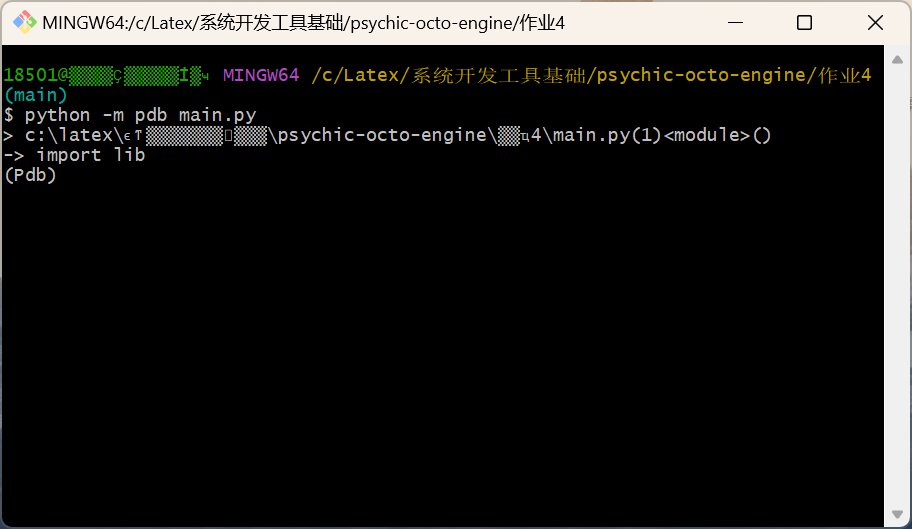
\includegraphics[width=14cm]{41d20ae257a69833fa1bf95d063eccf2.png}
        \caption{进入pdb}
        \label{fig:8}
        \end{figure}   
        \begin{figure}[H]
            \centering
            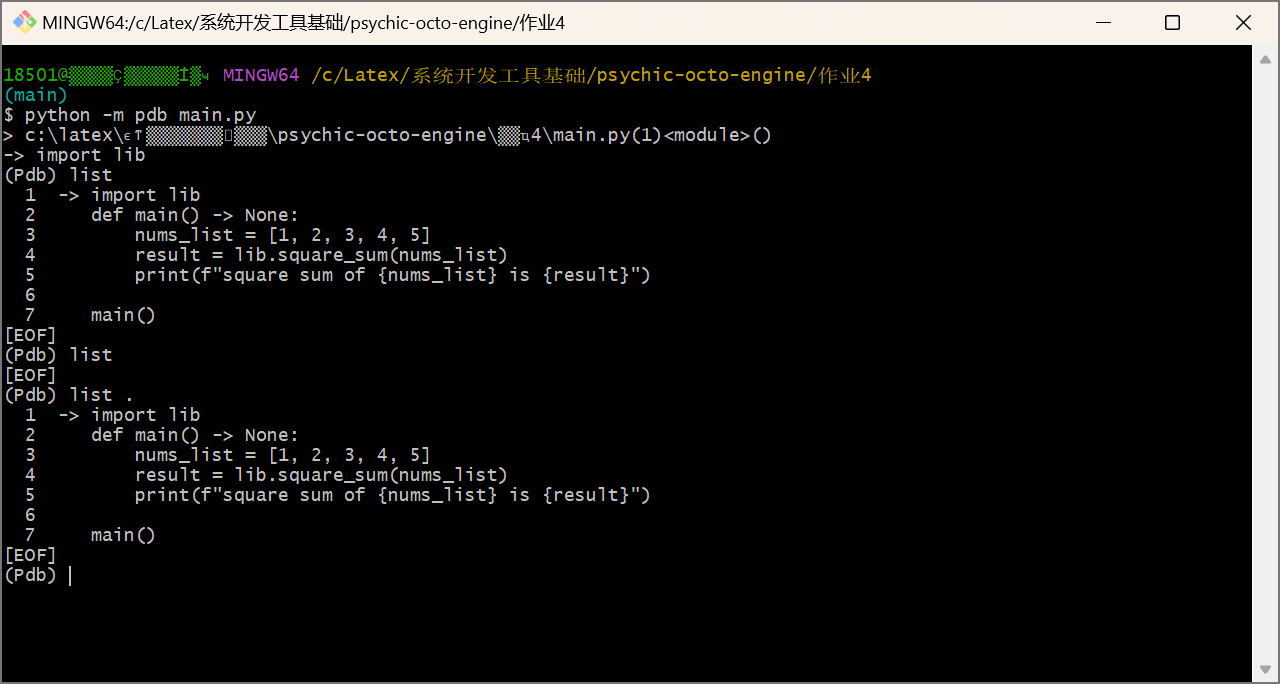
\includegraphics[width=14cm]{c7df9f2deb01459227251338902c74f6.png}
            \caption{list查看当前代码}
            \label{fig:9}
            \end{figure}   

        \begin{figure}[H]
            \centering
            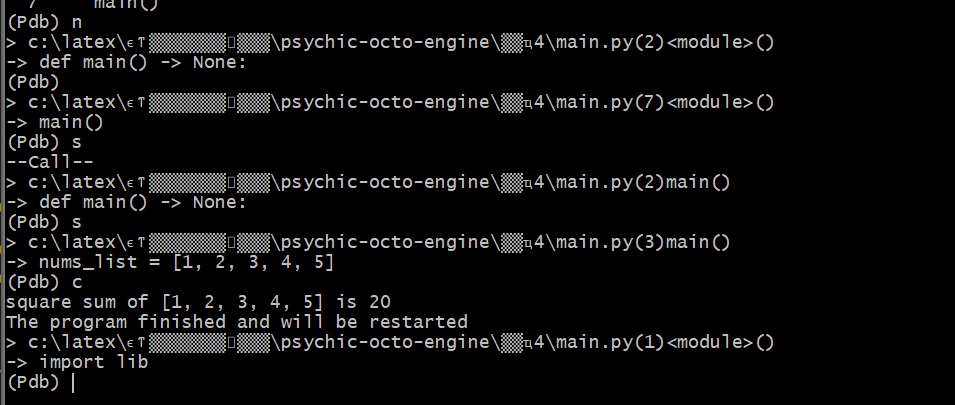
\includegraphics[width=14cm]{3063da819b46b90890b2c0e1296a91f2.png}
            \caption{n,s顺序查看代码,c结束代码}
            \label{fig:10}
            \end{figure}   
    4.我们先检查被调用的函数有没有出现问题,需要在函数内部设置断点:
    \begin{figure}[H]
        \centering
        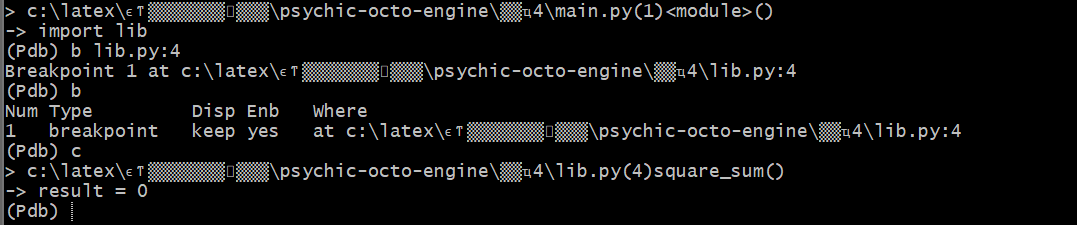
\includegraphics[width=14cm]{a3a391f7ff6e2a6b11844a5dfa5f5fdc.png}
        \caption{设置断点并进入到函数内部}
        \label{fig:11}
        \end{figure}   
    \begin{figure}[H]
        \centering
        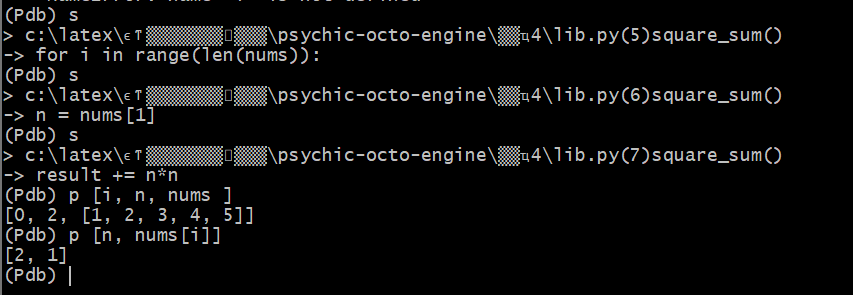
\includegraphics[width=14cm]{3ad352e05f8af1634160224f0329fad2.png}
        \caption{检查每个变量的值是否有问题}
        \label{fig:12}
        \end{figure}   
\begin{figure}[H]
        \centering
        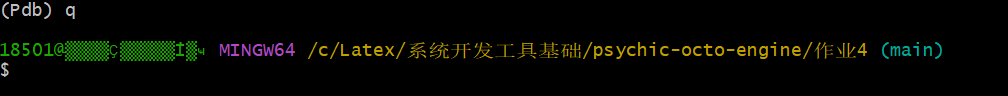
\includegraphics[width=14cm]{d96ee8d517b7678b97d1c7a750aaeaba.png}
        \caption{发现代码问题,修正并退出pdb}
        \label{fig:13}
        \end{figure}   
        \begin{figure}[H]
        \centering
        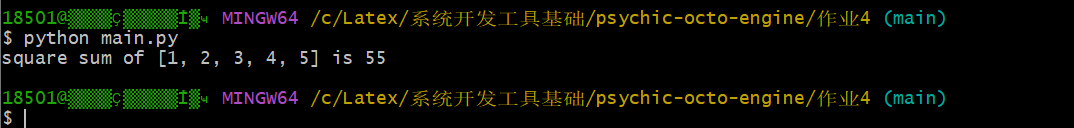
\includegraphics[width=14cm]{2a2e892688262f70ab14db9d9f4bac74.png}
        \caption{再运行代码,结果正确}
        \label{fig:14}
        \end{figure}   
\end{enumerate}


\subsection{元编程演示实验}
\begin{figure}[H]
    \centering
    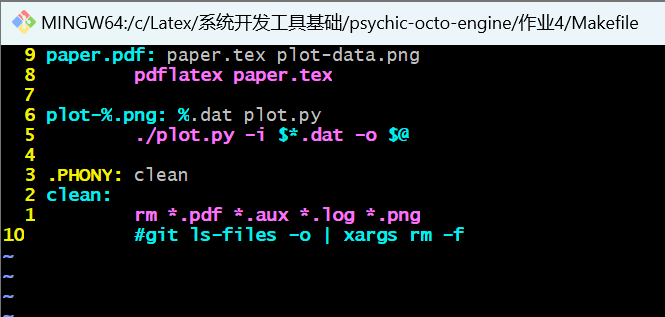
\includegraphics[width=14cm]{09f974d450731081da5f3ccb4bd1c0a4.png}
    \caption{编写代码}
    \label{fig:12}
    \end{figure}   
    \begin{figure}[H]
        \centering
        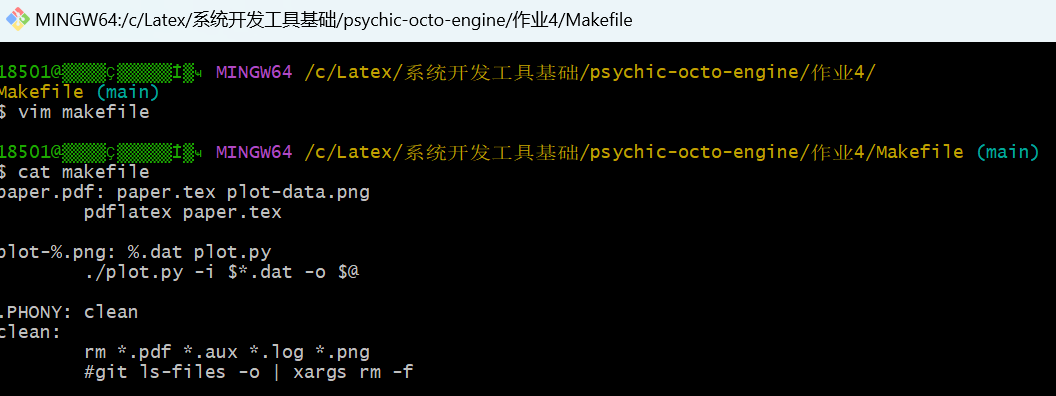
\includegraphics[width=14cm]{59f36beaa9e3ab13bc041dc5a0a419a5.png}
        \caption{cat展示}
        \label{fig:12}
        \end{figure}   
\section{实验心得}
\subsection{调试及性能分析}
我深刻认识到在编程中及时发现和解决问题的重要性。通过各种调试工具和技巧,我们能够精准地定位代码中的错误和瓶颈,
这不仅提高了代码的质量,更确保了程序的稳定运行。性能分析则让我学会了如何优化代码,使其在资源利用和运行效率上达到更优的状态,
这种对细节的关注和不断改进的追求让我在编程能力上有了显著的提升。

\subsection{元编程}
元编程展现出了编程领域极高的灵活性和创造性。它就像是一把神奇的钥匙,打开了通往更高级编程境界的大门。
在这个过程中,我们见识到了如何通过精妙的代码设计和巧妙的编程技巧,实现一些看似不可能的功能和行为。
例如,利用元编程可以动态地生成代码结构,根据特定的条件和需求在运行时构建合适的代码片段,这极大地拓展了程序的适应性和智能性。
它让我们能够深入探究编程的底层机制,不再仅仅满足于表面的代码编写,而是真正理解代码背后的运作原理。
这种对编程本质的更深入理解,激发了我探索更多编程可能性的强烈热情。我开始思考如何运用元编程的理念和方法,去创造更独特、高效的解决方案,
去突破传统编程思维的局限,去挖掘那些隐藏在代码世界深处的宝藏。

\subsection{PyTorch 编程}它强大的功能和简洁的接口使得构建深度学习模型变得相对容易和直观。
在使用 PyTorch 的过程中,我逐渐掌握了如何搭建复杂的神经网络结构、进行高效的训练和优化。
它让我切实感受到了深度学习的魅力和潜力,也让我对未来在这一领域的深入探索充满了期待。\\


总之,这一系列的学习经历让我受益匪浅。它们不仅丰富了我的知识体系,
更锻炼了我的思维能力和实践能力。我深知这些宝贵的经验将在我未来的编程道路上发挥重要的作用,激励我不断追求卓越,探索更多未知的领域。
\section{Github仓库ssh链接}
 \url {git@github.com:xixiyhaha/psychic-octo-engine.git }
\end{document}